\subsection{The Web Application}
We will be utilizing AWS' Amplify Console to host our web application which will allow users to view
the data and air quality information collected from the network of sensor nodes. We will be
designing this web application using the JavaScript framework, ReactJS, along with Typescript. Users
will be able to view one or many sensor data map overlays, and can toggle specific overlays, such as
\sdo or \ndo to hide or view them simultaneously. An account won't be required to view sensor data,
but an account will be required to setup a personal node. Users that are owners of sensor nodes will
be able to manage their devices, get detailed status information, and control them remotely through
a graphical (web) user interface or text console. A prototype of how the website might generally
look is shown in figures \ref{fig:website-prototype-map} and \ref{fig:website-prototype-map-dark}. 

\begin{figure}
    \centering
    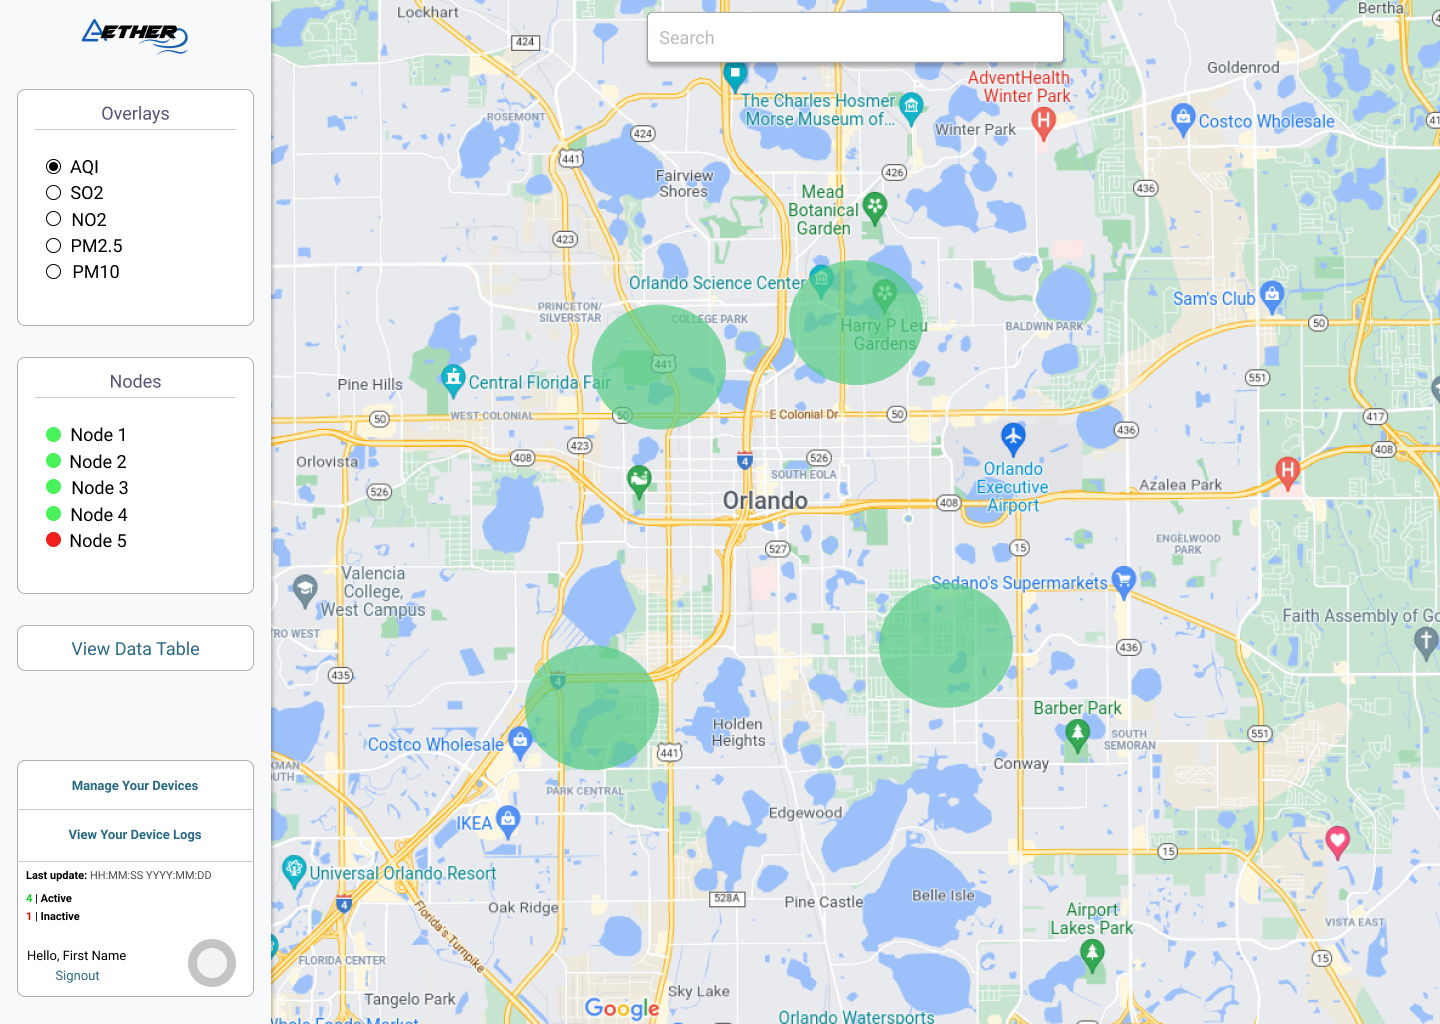
\includegraphics[width=6in]{webapp-prototype}
    \caption{Website Map View Prototype}
    \label{fig:website-prototype-map} 
\end{figure}

\begin{figure}
    \centering
    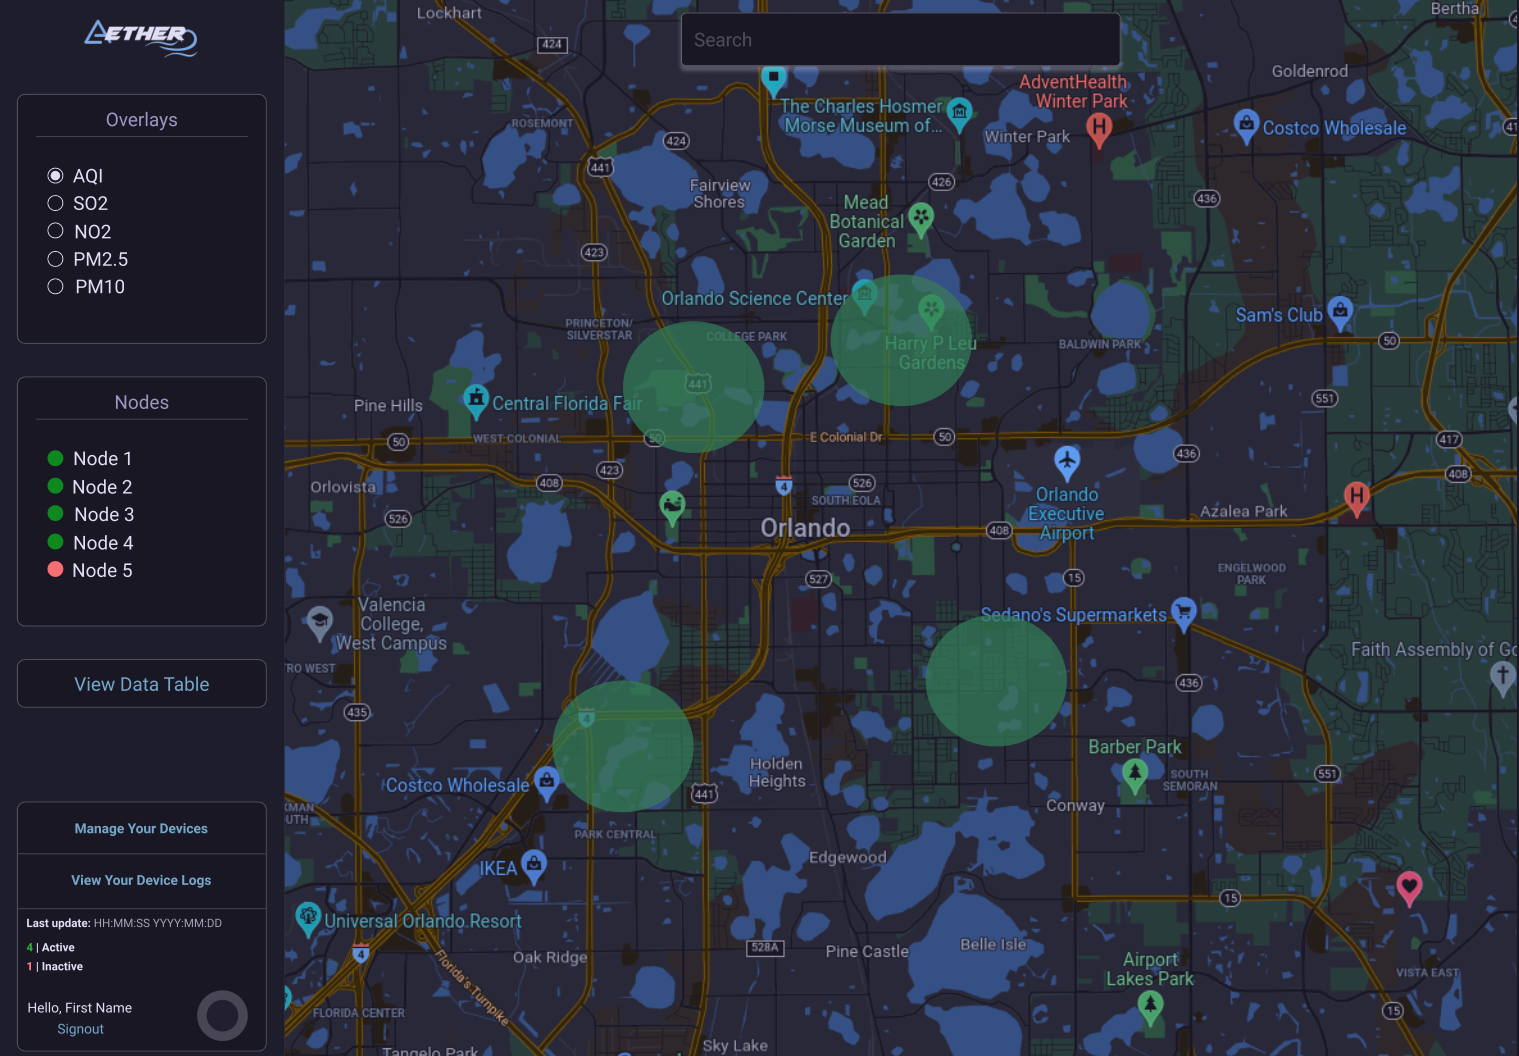
\includegraphics[width=6in]{webapp-prototype-dark}
    \caption{Website Map View Prototype - Dark Mode}
    \label{fig:website-prototype-map-dark} 
\end{figure}
